\documentclass{article}
\usepackage{graphicx}
\usepackage{float}
\usepackage{booktabs}
\usepackage{siunitx}

\title{Lab 2: Getting started with Ohm's Law, KVL, KCL, and Multi-Meter
Measurements}
\author{Sean Balbale}
\date{September 9th, 2023}
\setlength{\parindent}{0in}

\begin{document}

\begin{titlepage}
    \begin{center}
        \vspace*{1in}
            
        \Huge
        \textbf{Lab 2}
            
        \LARGE
        Getting started with Ohm’s Law, KVL, KCL, and Multi-Meter Measurements
            
        \vspace{3 in}
            
        \textbf{Student Name:} Sean Balbale
        \\ \textbf{Instructor:} Dr. Iman Salama
        \\ \textbf{Lab Partner Name:} Krish Gupta
        \\ \textbf{Date:} September 9th, 2024

        \vfill
            
            
    \end{center}
\end{titlepage}

\newpage 


\section{Introduction}
The lab had a few primary purposes: practicing Ohm’s law, 
KVL (Kirchhoff's voltage law), and KCL (Kirchhoff's current law), 
and learning how to use a Multimeter. The Keysight power supply 
and digital multimeter were used in this lab, which taught a 
necessary skillset for all electrical engineers.

\section{Results}


\subsection{A Very Simple DC Circuit}
\begin{figure}[H]
    \centering
    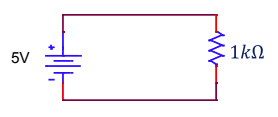
\includegraphics[width=0.5\textwidth]{simple_resistor_circuit_for_part1.png}
    \caption{Second Circuit built on breadboard. The red wires and rail are +6V while the black wire and blue rail are ground.}
    \label{fig:fig1}
\end{figure}

During this lab section, a very simple circuit (Figure~\ref{fig:fig1}) was built on a 
breadboard.  

\begin{figure}[H]
    \centering
    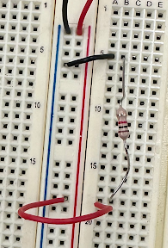
\includegraphics[angle=90,origin=c,width=0.5\textwidth]{built_figure1.png}
    \caption{Second Circuit built on breadboard. The red wires and rail are +6V while the black wire and blue rail are ground.}
    \label{fig:fig2}
\end{figure}

Figure~\ref{fig:fig2} shows the circuit that was built.
The theoretical amperage flowing through the resistor can be calculated
using Ohm's Law. This calculation is shown in Equation (1).

\begin{equation}
    I = \frac{V}{R}
    \text{, where } V = 5V \text{ and } R = 1k\Omega
\end{equation}

The actual value of the resistor used was found to be $1.0004 \: k\Omega$. When 
connected to a multimeter the voltage drop was measured to be $4.9986 \: V$.
The loop current was measured to be $4.9942 \: mA$. The measured values were close to the
calculated values, which is expected due to the accuracy of the equipment used.
The discrepancy between the calculated and measured values can be attributed to the
tolerance of the resistor and the accuracy of the multimeter. If the voltage over the
resistor doubles then, so will the loop current.

\subsection{KCL}


\section{Discussions and Conclusions}


\section{References}
[1] Dr. Iman Salama. “Lab 2 – Getting started with Ohm’s Law, KVL, KCL, 
and Multi-Meter Measurements” Northeastern University. 9 September 2024.

\end{document}
